\section{Conclusion}
\subsection{Summary of work}
The key findings, developments and tools built during the course of the project can be summarized as follows:
\begin{itemize}
\item An innovative way of performing system level tests using functional, regression, repository and performance testing techniques
\item An extensible DSL for functional, performance and regression testing on a system level
\item An extensible DSL for repository level testing in Scala
\item An extensible DSL for repository level testing in Python for comparison purposes.
\item API Wrappers for Mercurial
\item Various techniques and design patterns for embedded DSL implementation were explored and used
\end{itemize}

\subsection{Goals achieved}
The following goals were achieved over the course of the final year project:
\begin{itemize}
\item Different approaches towards developing a scalable DSL were explored
\item An embedded DSL for system testing was developed using Scala
\item 4 applications of the system were found - \textbf{HIP Verification, SLEEK verification and Regression Testing}
\item A DSL was developed in Python and Scala which can test all branches/commits of a mercurial project and summarize the results in an organized manner
\item This reporting tool is highly configurable using a YAML settings file.
\item The old system performing HIP/SLEEK testing was a 2500 line Perl Script. All the source code was translated using \textit{source code translators in Python} to the DSL code.
\end{itemize}

\subsection{Innovation}
There are several unit testing and web testing frameworks present in the software testing ecosystem today. However, there are very few tools that perform system level tests. The DSLs implemented fill in this gap in the testing ecosystem by providing flexible ways of performing regression, functional and performance testing. The \textbf{Repository Testing} feature provided is an innovative and effective technique to test the source code repository when several developers are contributing to it.

\subsection{Possible Areas of Extension}
There are several areas of extension and improvement for the DSL developed over the last year. Some of these possible improvements are:
\begin{itemize}
\item Improvement of Performance Testing features including graphical user interfaces
\item Cleaner syntax that abstracts away more details of host language, Scala
\item Run - time performance optimization through some meta - programming
\item Integrate \textbf{Git, SVN} or other version control tools with the reporting tool in Python
\item Extension of DSL to make it more generic and applicable to different applications for system testing
\end{itemize}

\subsection{Project Statistics}

Some interesting statistics during the development process are:
\begin{itemize}
\item 80\% of the project is written in Scala
\item 10\% of the project is written in Python
\item The remaining 10\% comprises setup scripts, configuration files and documentation
\item The total number of lines of code in the system are approximately 10,000
\item The project has 7 branches and 218 commits in the master branch
\end{itemize}

A graph showing commit frequency between September and April is shown below:
\begin{figure}[H]
  \centering
    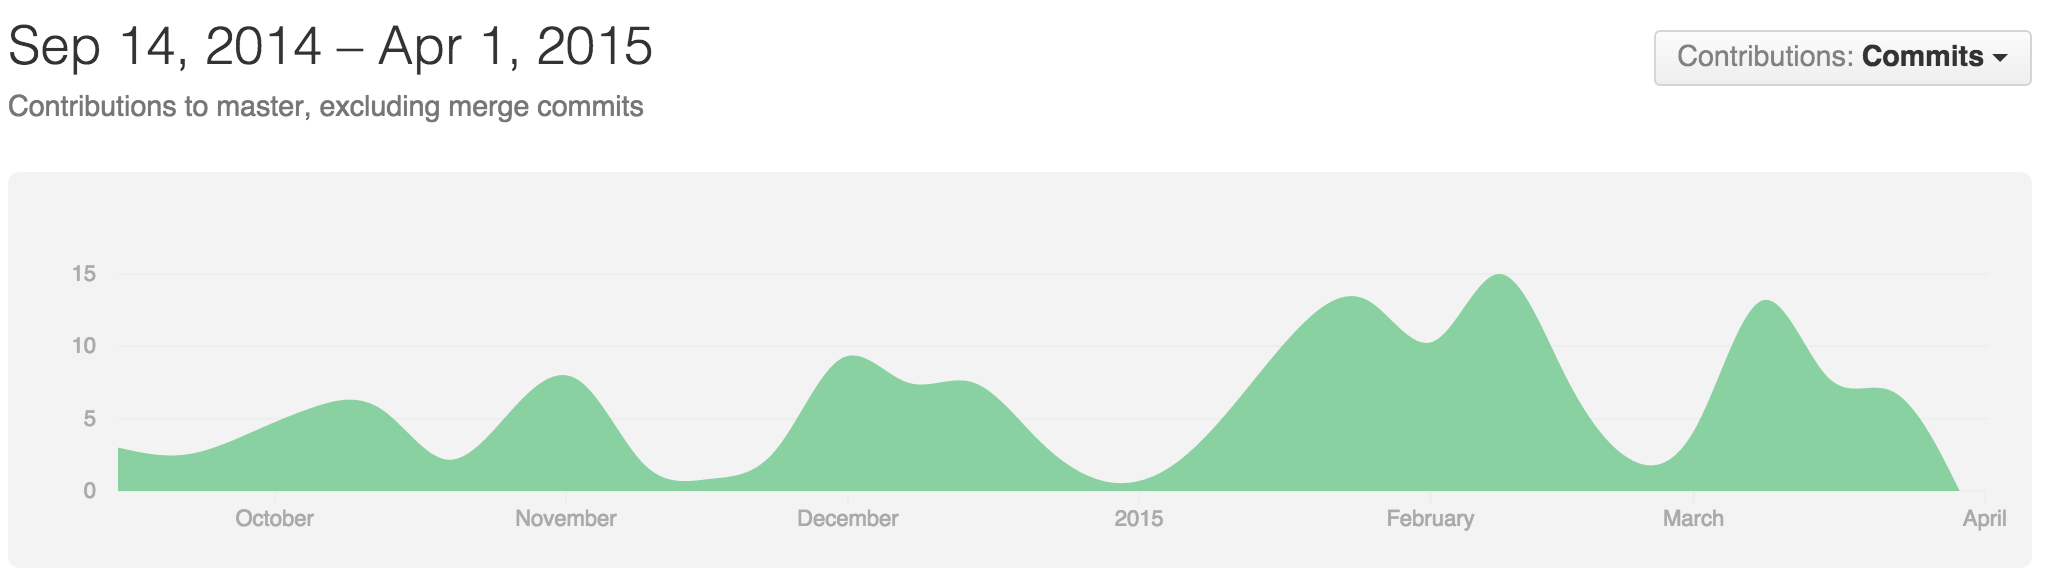
\includegraphics[height=120px]{figures/commit_frequency.png}
  \caption{Commit frequency statistics generated by Github}
\end{figure}
\newpage